\begin{enumerate}
 \item La fonction est définie dans $\R$ car $\frac{1-x^2}{1+x^2}$ et $\frac{2x}{1+x^2}$ sont dans $[-1,1]$. En effet :
\begin{align*}
 \frac{1-x^2}{1+x^2}-1 &= \frac{-2x^2}{1+x^2}\leq 0 &   \frac{1-x^2}{1+x^2}+1&=\frac{2}{1+x^2} \geq 0\\
 \frac{2x}{1+x^2}-1 &= -\frac{(1-x)^2}{1+x^2}\leq 0 &   \frac{(1+x)^2}{1+x^2}+1 &\geq 0 
\end{align*}
\item \begin{enumerate}
 \item On utilise les formules de cours 
\begin{align*}
 \arccos (-u) = \pi -\arccos u & & \arcsin (-u )= -\arcsin u
\end{align*}
\item En combinant les relations précédentes, on obtient
\begin{displaymath}
\left.
\begin{aligned}
 f(\frac{1}{x})&=\arccos\left(-\frac{1-x^2}{1+x^2} \right) +\arcsin\frac{2x}{1+x^2}\\
f(-x)&=\arccos\frac{1-x^2}{1+x^2} +\arcsin\left(-\frac{2x}{1+x^2} \right) 
\end{aligned}
\right\rbrace \Rightarrow
 f(\frac{1}{x}) + f(-x) = \pi
\end{displaymath}
\end{enumerate}
\item On reconnait les formules donnant le $\sin$ et le $\cos$ en fonction des $\tan$ de la moitié. On a donc, pour $x= \tan \theta$ :
\begin{align*}
 \frac{1-x^2}{1+x^2}= \cos (2\theta) & & \frac{2x}{1+x^2}= \sin (2\theta)
\end{align*}
\item On pose $\theta = \arctan x$ et on exprime $f(x)$ dans quatre cas selon le tableau suivant :
\renewcommand{\arraystretch}{1.7}
\begin{displaymath}
\begin{array}{c|c|c|c|c}
 x & ]-\infty,-1] & [-1,0] & [0,1] & [1,+\infty[  \\ \hline
 \theta & ]-\frac{\pi}{2},-\frac{\pi}{4}]  & [-\frac{\pi}{4},0] & [0,\frac{\pi}{4}] & [\frac{\pi}{4},\frac{\pi}{2}[ \\ \hline
 2\theta & ]-\pi ,-\frac{\pi}{2}]  & [-\frac{\pi}{2},0] & [0,\frac{\pi}{2}] & [\frac{\pi}{2},\pi[ \\ \hline
 \arccos (\cos (2\theta)) & -2\theta & -2\theta & 2\theta & 2\theta \\ \hline
 \arcsin (\sin (2\theta)) & -\pi -2\theta & 2\theta & 2\theta & \pi -2\theta \\ \hline
 f(x) & -\pi - 4\arctan x & 0 & 4\arctan x & \pi
\end{array}
\end{displaymath}
On en déduit le graphe de $f$ (figure \ref{fig:Celem9_1}). On aurait pu se limiter aux deux intervalles dans $\R_+$ et obtenir les autres expressions avec le résultat de 2.b.
\end{enumerate}
\begin{figure}[h!t]
 \centering
 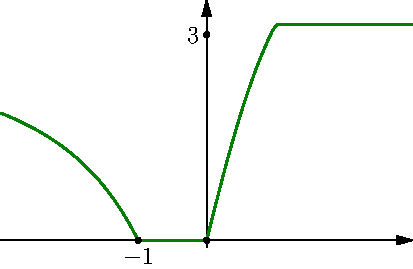
\includegraphics[width=7cm]{Celem9_1.pdf}
 \caption{Graphe de $\arccos \left(\frac{1-x^2}{1+x^2}\right) + \arcsin \left( \frac{2x}{1+x^2}\right)$}
 \label{fig:Celem9_1}
\end{figure}
